\documentclass[12pt]{article}
\usepackage{../light}

\hidesolutions
%\showsolutions

\newcommand{\edge}[2]{#1\text{---}#2}
\newcommand{\mfigure}[3]{\bigskip\centerline{\resizebox{#1}{#2}{\includegraphics{#3}}}\bigskip}

\begin{document}

\recitation{12}{October 20, 2010}

%%%%%%%%%%%%%%%%%%%%%%%%%%%%%%%%%%%%%%%%%%%%%%%%%%%%%%%%%%%%%%%%%%%%%%%%%%%%%%%

\newcommand{\bigbox}{\fbox{\vspace{0.5in} \hspace{0.75in}}}

\section{The L-tower problem}

%% Prof Leighton suggests the following changes: as part of the question, we should ask them to figure out what the condition on x is for near instabiility. We can also ask for a condition on x for when it is most stable. The latter is when x is close to an even integer. 

Observe the structures shown in Figure~\ref{fig:towers}.  One has 2 L-shapes, the other 5 L-shapes. Consider a tower with $k$ L-shapes.  Assume that the blocks are all of size $x\times 1$ where $x > 1$. As the picture indicates,  if $k$ is too small then the tower falls to the left. On the other hand, if $k$ is too large the tower would fall to the right. Will the tower be stable for some $k$?  Prove there is at least one value of $k$ for which the L-tower is stable.  Assume that a structure is stable if and only if its center of gravity is not hanging in the air horizontally. The L-tower is stable if and only if each of its subparts is stable.   \\

\emph{Hint:}  Show the tower is stable if and only if $\frac{3x - 3}{2} \leq  k \leq \frac{3x - 1}{2} $.

\begin{figure}[h]

\centering
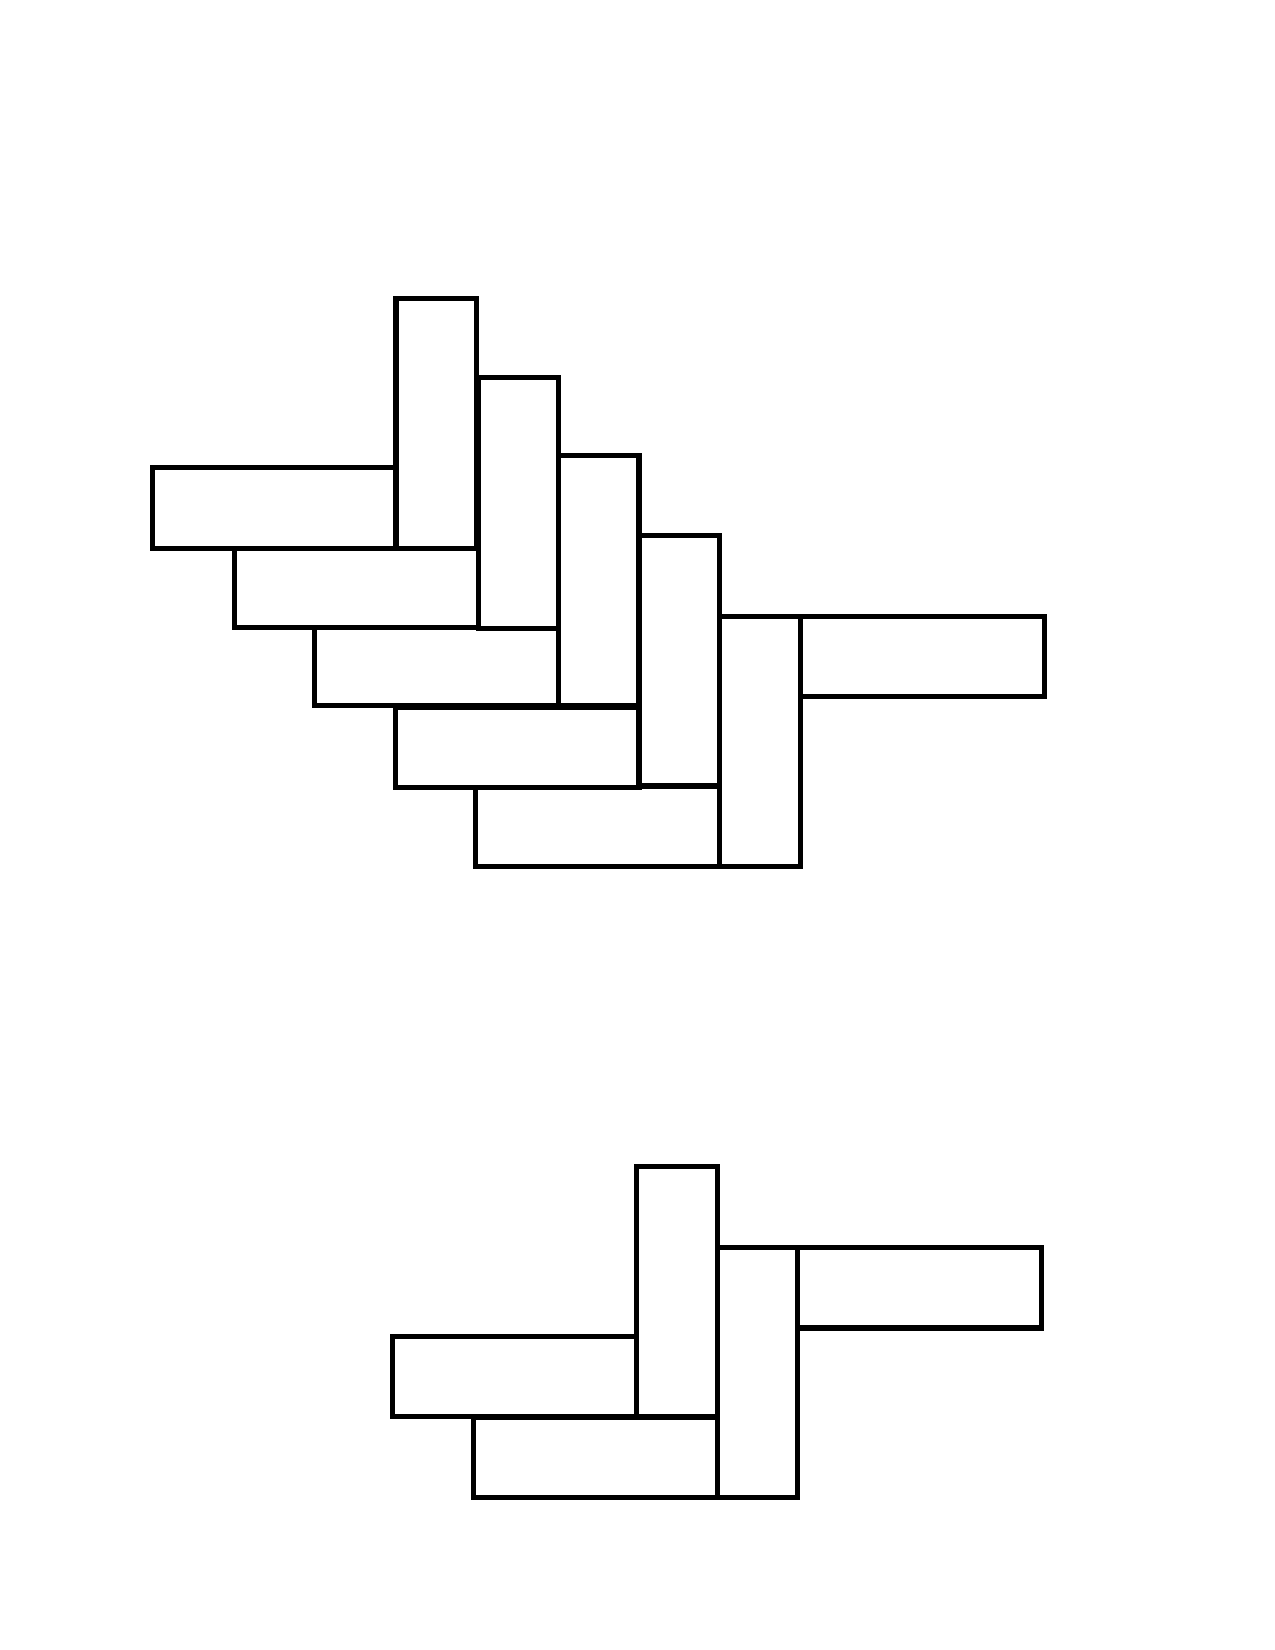
\includegraphics[scale=0.4, angle=-90]{Diagram1}
\caption{Too few or too many L shapes make the tower unstable \label{fig:towers}}
\end{figure}

\solution{
As indicated in the description, an arbitrary structure is considered stable if and only if its center of gravity lies on top of some form of support. For our L-towers this implies several conditions that must hold simultaneously. Consider the case $k=3$, illustrated in Figure~\ref{fig:conditions}. For the structure to be stable, we need the topmost L-shape to be stable on top of the second L-shape.  This is Condition 1.  We also need the structure formed by the topmost 2 L-shapes to be overall stable on top of the lowest L-shape. This is Condition 2. And finally, we need the three L-shapes to be stable on top of the single standing block. Call this Condition 3. In general, if there are $k$ L-shapes, there are $k$ conditions that must be satisfied for the structure to be stable. We will explicitly describe these constraints below.

\begin{figure}
\centering
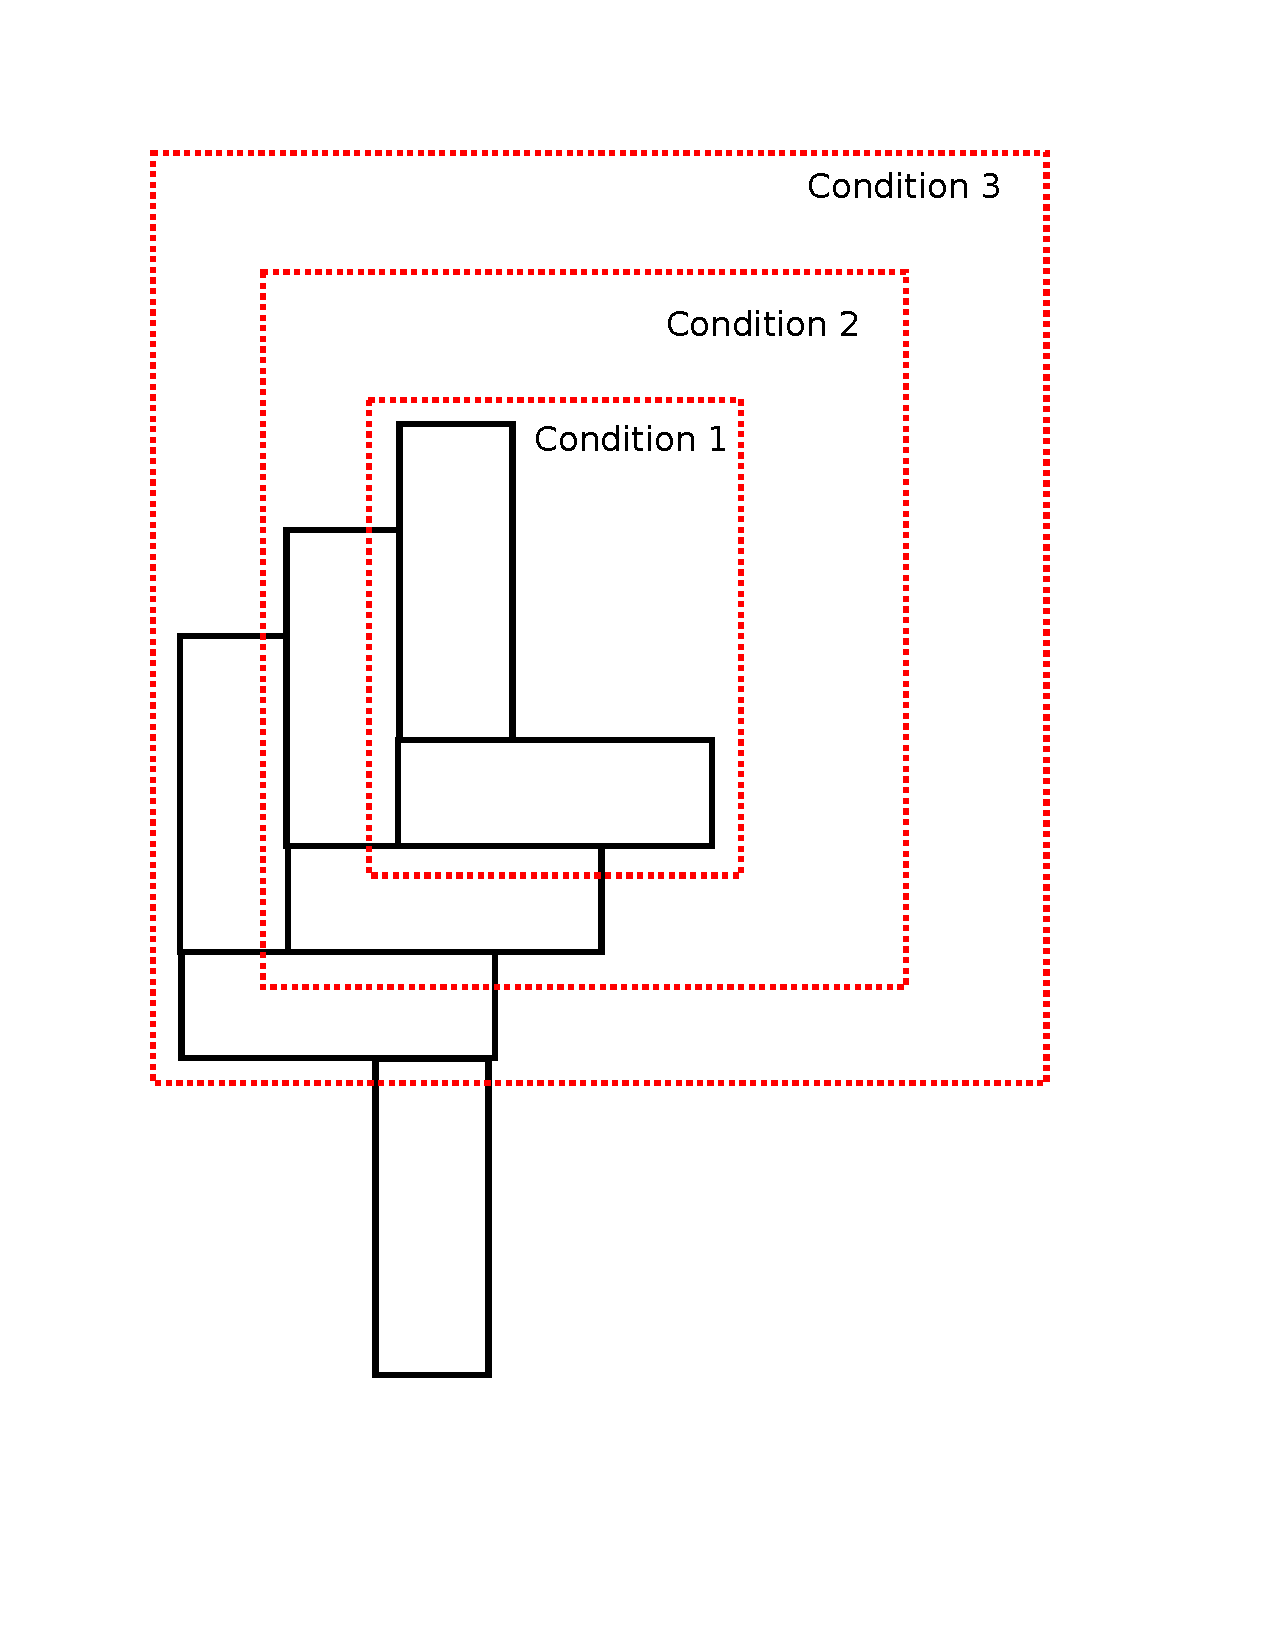
\includegraphics[scale = 0.4]{sol1}
\caption{Three necessary conditions for stability, when $k = 3$ \label{fig:conditions}. Put together, we also consider them sufficient.}
\end{figure}

Throughout the solution we are only concerned with the x-coordinates of the center of mass. The center of mass of a set of L-shapes can be computed by partitioning the figure into individual L shapes, and then averaging their individual centers. 

Let $c_1$ be the position of the center of mass for an individual L-shape starts at $0$. The vertical block has its center at $1/2$, the horizontal block at $x/2$. Hence, the center of a single L-shape is $(1/2 + x/2)/2 = (x + 1)/4$ to the right of where it starts.

Now let $c_h$ be the position for the center of mass of $h$ L-shapes stacked together, where we have shifted our reference frame so that the structure starts at $0$. This new center of mass can be obtained from averaging the center of a single L shaped shifted by 1 every time. So we get $c_h = \left[ c_1 + (c_1 + 1) + \cdots + (c_1 + (h -1))\right] / h$.  Regrouping, we get $c_h  = \left[ hc_1 + (1 + 2 + \cdots + (h-1)) \right] / h = \left[ hc_1 + h(h-1)/ 2 \right] /  h$, from where we arrive to: $c_h = c_1 + (h-1)/2$. 
It is helpful to think visually about this equation. When $h=1$, we naturally get $c_h = c_1$. As $h$ increases, the center shifts by $1/2$ to the right every time.

Now we can write explicitly all the conditions for a structure  with $k$ L-shapes to be stable. We need every structure to stand stable on top of the next L. If we imagine we have a stack of $i$ L-shapes starting at 0 on top of another L-shape starting at $-1$, we require:

$$c_i \leq x - 1$$

This simply means that if we have a stack of $i$ L-shapes starting right on the origin, we need its center of gravity to fall within the next L. The next L ends at $x-1$.

If we have $k$ L-shapes, this constraint applies to the first $k-1$ stacks. So we get the conditions:

$$c_1 \leq x-1$$
$$c_2 \leq x-1$$
$$\vdots$$
$$c_{k-1} \leq x-1$$

Finally, the overall stack of $k$ L-shapes has a slightly different requirement, since it stands on top of the vertical block:

$$x - 1 \leq  c_{k} \leq x$$

Now we need to find whether some $k$ satisfies all of these constraints. Recall $c_{k-1} > c_{k-2} > \cdots > c_{1}$, so we only need to check the last two constraints $c_{k-1} \leq x -1$ and $x - 1 \leq  c_{k} \leq x$. Substituting $c_k = (x+1)/4  + (k - 1)/2$ and $c_{k-1} = c_{k} - 1/2 = (x + 1)/4 + (k-1)/2 - 1/2$, we get the inequalities:

$$(x + 1)/4 + (k-1)/2 \leq  x - 1/2$$
$$ x - 1 \leq (x+1)/4 + (k-1)/2 \leq x$$

The first inequality is stronger on the right than the second, so consolidating both we get:

$$ x - 1 \leq  (x+1)/4 + (k-1)/2 \leq x - 1/2$$ which solved for $k$ yields:

$$\dfrac{3x - 3}{2} \leq k \leq \dfrac{3x- 1}{2}$$

There is a gap between the upper and lower bound of exactly 1. Hence either there is an integer right between them, or both are integers. For $(3x-3)/2$ to be an integer we need $x$ to be an odd integer.  Hence in the case where $x$ is an odd integer we have two choices of $k$ but on each the structure will be barely stable.

}
%%%%%%%%%%%%%%%%%%%%%%%%%%%%%%%%%%%%%%%%%%%%%%%%%%%%%%%%%%%%%%%%%%%%%%%%%%%%%%%
\newpage

\section{Double Sums}

Sometimes we have to evaluate sums of sums, otherwise known as
\emph{double summations}. It's good to know how to tame these beasts!
Here's an example of a double summation:
\[
\sum_{i=1}^n \sum_{j=1}^i j
\]
It looks ferocious...all those sharp teeth! But actually, this double
summation is just a sheep in wolf's clothing: to evaluate it, we can
just evaluate the inner sum, replace it with a closed form we already
know, and then evaluate the outer sum which no longer has a summation
inside it.

\begin{itemize}
\item Evaluate the summation. (\textit{Hint: $\sum(a+b)=\sum a + \sum b$.})

\solution[\vspace{3in}]{
\begin{align*}
\sum_{i=1}^n \sum_{j=1}^i j &= \sum_{i=1}^n \frac{i(i+1)}{2}\\
&= 1/2 \sum_{i=1}^n (i^2 + i)\\
&= 1/2(\sum_{i=1}^n i^2 + \sum_{i=1}^n i)\\
&= 1/2(\frac{n^3}{3} + \frac{n^2}{2} + \frac{n}{6} + \frac{n(n+1)}{2})\\
&= 1/2(\frac{n^3+3n^2+2n}{3})
\end{align*}
}
\end{itemize}

Unfortunately, not all summations are so docile. Fortunately, we have
ways to deal with this. There's a special trick that is often
extremely useful for sums, and that is to \emph{exchange the order of
  summation.}  We'll go through an example here.

For the remainder of the problem we'll wrestle with the sum of the
harmonic numbers:
\[
\sum_{k=1}^n H_k
\]
At first glance, it looks like just a single summation, but do not be
deceived.

\begin{itemize}

\item 
First, write it as a double summation.

\solution[\vspace{.5in}]{
\[
\sum_{k=1}^n H_k = \sum_{k=1}^n \sum_{j=1}^k 1/j
\]
}

\item 
Now try to gain some intuition for exactly what you're up against by
integrating the summation in its less threatening single-summation
form. You may use $H_k \approx \ln k$.

\solution[\vspace{.5in}]{
\[
\sum_{k=1}^n H_k \approx \int_{k=1}^n \ln n = n\ln n-n+1.
\]
}


\item Finally, we'll look for an exact answer. If we think about the
  pairs $(k,j)$ over which we are summing, they form a triangle in the
  table below. The values in the cells of the table correspond to the
  terms in the double summation. The first two rows have been filled
  in for you. Complete the remaining three rows to see the pattern.

\[
\begin{array}{c|cccccc}
j&1&2&3&4&\dots&n\\
\hline
k\\
1&1\\
2 &1&1/2\\
3 \\
4 \\
 &\dots\\
n &&&&&\dots
\end{array}
\]

\solution{
\[
\begin{array}{c|cccccc}
j&1&2&3&4&\dots&n\\
\hline
k\\
1&1\\
2 &1&1/2\\
3 &1&1/2&1/3\\
4 &1&1/2&1/3&1/4\\
 &\dots\\
n &1&1/2&1/3&1/4&\dots&1/n
\end{array}
\]
}

\item The summation above is summing each row and then adding the row
  sums.  But we can tame this beast if, instead, we first sum the
  columns and then add the column sums. Use the table to rewrite the
  double summation. The inner summation should sum over $k$, and the
  outer summation should sum over $j$.

\solution[\vspace{.5in}]{
\begin{align*}
\sum_{k=1}^n H_k &= \sum_{k=1}^n \sum_{j=1}^k 1/j\\
&= \sum_{j=1}^n \sum_{k=j}^n 1/j\\
\end{align*}
}

\item Now simplify the summation to derive a closed form in terms of
  $n$ and $H_n$.

\solution[\vspace{3in}]{
\begin{align*}
\sum_{k=1}^n H_k &= \sum_{j=1}^n \sum_{k=j}^n 1/j\\
&= \sum_{j=1}^n 1/j \sum_{k=j}^n 1\\
&= \sum_{j=1}^n \frac1j (n-j+1)\\
&= \sum_{j=1}^n \frac{n-j+1}j \\
&= \sum_{j=1}^n \frac{n+1}j - \sum_{j=1}^n \frac{j}{j}\\
&= (n+1)\sum_{j=1}^n \frac1j - \sum_{j=1}^n 1\\
&= (n+1)H_n-n
\end{align*}
Notice that the exact solution is very similar in form to the
approximation we generated above.
}

\end{itemize}
%% \section{Double Sums}
%% 
%% \begin{definition}\label{sig1}
%% \begin{align*}
%% \sum_{k=1}^{0}{f(k)} & = 0,   &\emph{(an empty sum)}\\
%% \sum_{k=1}^{n+1}{f(k)} & = f(n+1) + \sum_{k=1}^{n}{f(k)}.
%% \end{align*}
%% \end{definition}
%% 
%% 
%% Double (or triple, \dots) sums arise all the time.  Informally, we can
%% picture a double sum as:
%% \[\begin{array}{rcl}
%% \sum_{i=0}^{p}{\sum_{j=0}^{n}{f(i,j)}}
%%     = & \sum_{i=0}^{p}{(f(i,0)+ \cdots +f(i,n))}\\
%%     = & (f(0,0)+ \cdots  +f(0,n)) & +\\
%%       & (f(1,0)+ \cdots  +f(1,n)) & +\\
%%       &          \vdots           & +\\
%%       & (f(p,0)+ \cdots  +f(p,n)).
%% \end{array}\]
%% 
%% We mention one useful identity for double sums.
%% \[
%% \sum_{i=1}^{p}{\sum_{j=1}^{n}{(f(i) \cdot g(j))}}
%%  = \Big(\sum_{i=1}^{p}{f(i)} \Big) \Big(\sum_{j=1}^{n}{g(j)} \Big).
%% \]
%% The proof follows from Definition~\ref{sig1} by a couple of uses of the
%% Distributive Rule.  We'll skip the details.
%% 
%% \iffalse
%% In order to show that this formula is valid, we write down the definition
%% to find that:
%% \begin{align*}
%%   \sum_{i=0}^{p}{\sum_{j=0}^{n}{(f(i) \cdot g(j))}} & = (f(0)g(0)+ \cdots +f(0)g(n))+
%%   \cdots +(f(p)g(0)+ \cdots +f(p)g(n))\\
%%      & = f(0)(g(0)+ \cdots +g(n))+ \cdots +f(p)(g(0)+ \cdots +g(n))\\
%%      & = (f(0)+ \cdots +f(p))(g(0)+ \cdots +g(n))\\
%%      & = \Big(\sum_{i=0}^{p}{f(i)}\Big) \Big(\sum_{j=0}^{n}{g(j)}\Big)
%% \end{align*}
%% \fi
%% 
%% \begin{itemize}
%% 
%% %% Let's skip this -- I don't think we want to focus too heavily on sums in this course.
%% 
%% \item
%% \[
%% \sum_{i=0}^{p}{\sum_{j=0}^{n}{f(i,j)}}=\sum_{j=0}^{n}{\sum_{i=0}^{p}{f(i,j)}}.
%% \]
%% 
%% In order to compute a double sum, it might be easier to start summing one
%% set of indices before the other one. The following example illustrates
%% this point: ANYONE HAS A GOOD EXAMPLE?
%% \end{itemize}

%%%%%%%%%%%%%%%%%%%%%%%%%%%%%%%%%%%%%%%%%%%%%%%%%%%%%%%%%%%%%%%%%%%%%%%%%%%%%%%
%% NOTE: going on pset 7

%% \section{The Search for the Holy Grail???}
%% An explorer is trying to reach the Holy Grail, which she believes is
%% located in a desert shrine $d$ days walk from the nearest
%% oasis.\footnote{She's right about the location, but doesn't realize
%% that the Holy Grail is actually just the Bene\u{s} network.}  In the
%% desert heat, the explorer must drink continuously.  She can carry at
%% most 1 gallon of water, which is enough for 1 day.  However, she is
%% free to create water caches out in the desert.
%% 
%% For example, if the shrine were $2/3$ of a day's walk into the desert,
%% then she could recover the Holy Grail with the following strategy.
%% She leaves the oasis with 1 gallon of water, travels $1/3$ day into
%% the desert, caches $1/3$ gallon, and then walks back to the oasis---
%% arriving just as her water supply runs out.  Then she picks up another
%% gallon of water at the oasis, walks $1/3$ day into the desert, tops
%% off her water supply by taking the $1/3$ gallon in her cache, walks
%% the remaining $1/3$ day to the shine, grabs the Holy Grail, and then
%% walks for $2/3$ of a day back to the oasis--- again arriving with no
%% water to spare.
%% 
%% But what if the shrine were located farther away?
%% 
%% \begin{enumerate}
%% 
%% \item What is the most distant point that the explorer can reach and
%% return from if she takes only 1 gallon from the oasis.?
%% 
%% \solution[\vspace{0.75in}]{At best she can walk $1/2$ day into the
%% desert and then walk back.}
%% 
%% \item What is the most distant point the explorer can reach and
%% return form if she takes only 2 gallons from the oasis?  No proof is
%% required; just do the best you can.
%% 
%% \solution[\vspace{1in}]{The explorer walks $1/4$ day into the
%% desert, drops $1/2$ gallon, then walks home.  Next, she walks $1/4$
%% day into the desert, picks up $1/4$ gallon from her cache, walks an
%% additional $1/2$ day out and back, then picks up another $1/4$ gallon
%% from her cache and walks home.  Thus, her maximum distance from the
%% oasis is $3/4$ of a day's walk.}
%% 
%% \item What about 3 gallons?  (Hint: First, try to establish a cache
%% of 2 gallons \textit{plus} enough water for the walk home as far into
%% the desert as possible.  Then use this cache as a springboard for your
%% solution to the previous part.)
%% 
%% \solution[\newpage]{Suppose the explorer makes three trips $1/6$ day
%% into the desert, dropping $2/3$ gallon off units each time.  On the
%% third trip, the cache has 2 gallons of water, and the explorer still
%% has $1/6$ gllon for the trip back home.  So, instead of returning
%% immediately, she uses the solution described above to advance another
%% $3/4$ day into the desert and then returns home.  Thus, she reaches
%% %
%% \[
%% \frac{1}{6} + \frac{1}{4} + \frac{1}{2} = \frac{11}{12}
%% \]
%% %
%% days' walk into the desert.}
%% 
%% \item How can the explorer go as far as possible is she withdraws $n$
%% gallons of water?  Express your answer in terms of the Harmonic number
%% $H_n$, defined by:
%% %
%% \[
%% H_n = \frac{1}{1} + \frac{1}{2} + \frac{1}{3} + \ldots \frac{1}{n}
%% \]
%% 
%% \solution[\vspace{3in}]{With $n$ gallons of water, the explorer can
%% reach a point $H_n / 2$ days into the desert.
%% 
%% Suppose she makes $n$ trips $1/(2n)$ days into the desert, dropping of
%% $(n-1)/n$ gallons each time.  Before she leaves the cache for the last
%% time, she has $n-1$ gallons plus enough for the walk home.  So she
%% applies her $(n-1)$-day strategy to go an additional $H_{n-1} / 2$
%% days into the desert and then returns home.  Her maximum distance from
%% the oasis is then:
%% %
%% \[
%% \frac{1}{2n} + \frac{H_{n-1}}{2} = \frac{H_n}{2}
%% \]
%% }
%% 
%% \item Use the fact that
%% %
%% \[
%% H_n \sim \ln n
%% \]
%% %
%% to approximate your previous answer in terms of logarithms.
%% 
%% \solution[\vspace{1in}]{An approximate answer is $\ln n / 2$.  }
%% 
%% \item Suppose that the shrine is $d = 10$ days walk into the desert.
%% Relying on your approximate answer, how many days must the explorer
%% travel to recover the Holy Grail?
%% 
%% \solution{
%% She can obtains the Grail when:
%% %
%% \[
%% \frac{H_n}{2} \approx \frac{\ln n}{2} \geq 10
%% \]
%% %
%% This requires about $n \geq e^{20} = 4.8 \cdot 10^8$ days.
%% }
%% 
%% \end{enumerate}

%%%%%%%%%%%%%%%%%%%%%%%%%%%%%%%%%%%%%%%%%%%%%%%%%%%%%%%%%%%%%%%%%%%%%%%%%%%%%%%

\end{document}
